%!TeX ts-program = xelatex
%!TeX encoding = utf-8 Unicode
\documentclass[ieeetran]{article}
\usepackage{amsmath, amssymb}
\usepackage{graphicx}
\usepackage{tikz}
\usetikzlibrary{automata,positioning}

\title{Einführung in die Theoretische Informatik Zusammenfassung}
\author{Efe Kamasoglu}

\begin{document}

\maketitle

\pagebreak

\section{Grundbegriffe und Grammatiken} % (fold)
\label{sub:grundbegriffe_und_grammatiken}

\subsection{Grundbegriffe} % (fold)
\label{sub:grundbegriffe}
\begin{itemize}
  \item Alpabet $\Sigma$, endliche Menge
  \item Wort/String $w$ über $\Sigma$, endliche Menge von Zeichen aus $\Sigma$
\item $|w|$, Länge des Wortes $w$
\item $\epsilon$, das leere Wort mit der Länge 0
\item Wörter $u$ und $v$, $uv$ ist ihre Konkatenation
\item Wort $w$, $w^n$ definiert durch:
	\begin{itemize}
	  \item $w^0 = \epsilon$
	  \item $w^{n + 1} = ww^n$
	  \item \textit{\underline{Beispiel:} $(ab)^3 = ababab$}
         
	\end{itemize}

\item $\Sigma ^*$, Menge aller Wörter über $\Sigma$
\item Teilmenge $L \subseteq \Sigma ^*$, formale Sprache
	\begin{itemize}
		\item \textit{\underline{Beispiel:} $\emptyset$, $\{\epsilon\}$, $L_1 = \{\epsilon, ab, aabb, aaabbb, ... \} = \{a^nb^n \ | \ n \in \mathbb{N} \}$}
	\end{itemize}
\end{itemize}

\subsection{Operationen auf Sprachen} % (fold)
\label{sub:operationen_auf_sprachen}
Sprachen $A, B \subseteq \Sigma ^*$

\begin{itemize}
	\item \textbf{Konkatenation:} $AB = \{uw \ | \ u \in A \ \wedge \ w \in B \}$
		\begin{itemize}
			\item \textit{\underline{Beispiel:}} $\{ab,b\}\{a,bb\} = \{aba, abbb, ba, bbb\}$
			\item $A^n = \{w_1...w_n \ | \ w_1,...,w_n \in A\} = \underbrace{A...A}_\text{n}$
			\item $A^0 = \{ \epsilon \}, \ A^{n+1} = AA^n$
			\item $A^* = \{w_1...w_n \ | \ n \ge 0 \ \wedge \ w_1,...,w_n \in A\} = \bigcup_{n \in \mathbb{N}}A^n$
				\begin{itemize}
					\item $A^*$ enthält $\epsilon$ immer
				\end{itemize}
			\item $A^+ = AA^* = \bigcup_{n \ge 1}A^n$
				\begin{itemize}
				  \item $\epsilon \in A \ gdw. \ \epsilon \in A^+$
				\end{itemize}

		\end{itemize}
	\item \textbf{Kartesisches Produkt:} $A \times B$
		\begin{itemize}
			\item \textit{\underline{Beispiel:}} $\{ab,b\} \times \{a,bb\} = \{(ab,a),(ab,bb),(b,a),(b,bb)\}$
		\end{itemize}
	
\item \textbf{Rechenregeln über Sprachen:}
	\begin{itemize}
		\item Für alle $A$: $\epsilon \in A^*$
	\item $\epsilon \not\in \emptyset$
	\item $\emptyset^* = \{\epsilon\} = \emptyset^0$
	\item $A\{\epsilon\} = \{\epsilon\}A = A$
	\item $A\emptyset= \emptyset A = \emptyset$
	\item $A \times \emptyset = \emptyset$
	\item $A(B \cup C) = AB \cup AC$
	\item $(A \cup B)C = AC \cup BC$
	\item $A(B \cap C) = AB \cap AC$ gilt i.A. \textbf{nicht}
	\item $A(B \setminus C) = AB \setminus AC$ gilt i.A. \textbf{nicht}

	\item $A^*A^* = (A^*)^* = A^*$
	\end{itemize}
\end{itemize}

\subsection{Grammatiken} % (fold)
\label{sub:grammatiken}
\begin{itemize}
	\item Grammatik, 4-Tupel $G = (V, \Sigma, P, S)$
\begin{itemize}
	\item $V$, endliche Menge von \textbf{Nichtterminalen}
	\item $\Sigma$, endliche Menge von \textbf{Terminalen}, disjunkt von $V$
	\item $P \subseteq (V \cup \Sigma)^* \times (V \cup \Sigma)^*$, Menge von \textbf{Produktionen}
	\item $S \in V$, \textbf{Startsymbol}
\end{itemize} 

\item Eine Grammatik G induziert eine \textbf{Ableitungsrelation} $\rightarrow_G$ auf Wörtern über $V \cup \Sigma$:
\begin{itemize}
  \item $\alpha \rightarrow \alpha'$ gdw.\ es eine Regel $\beta \rightarrow \beta'$ in $P$ und Wörter $\alpha_1, \alpha_2$ gibt, so dass $\alpha = \alpha_1 \beta \alpha_2 \ \wedge \ \alpha' = \alpha_1 \beta' \alpha_2$
\end{itemize}

\item Eine \textbf{Sequenz} $\alpha_1 \rightarrow_G \alpha_2 \rightarrow_G ... \rightarrow_G \alpha_n$ ist eine \textbf{Ableitung} von $\alpha_n$ aus $\alpha_1$.
\item Wenn $\alpha_1 = S$ und $\alpha_n \in \Sigma^*$, dann \textbf{erzeugt} $G$ das Wort $\alpha_n$.\ Erzeugte Wörter bestehen nur aus \textbf{Terminalzeichen}.

\item Die Sprache von $G$ ist die Menge aller Wörter ($\Sigma^*$), die von $G$ erzeugt werden: $L(G)$

\item \textbf{Chomsky Hierarchie:} Eine Grammatik $G$ ist vom
\begin{itemize}
  \item \textbf{Typ 0} immer
\item \textbf{Typ 1} falls für jede Produktion $\alpha \rightarrow \beta$ ausser $S \rightarrow \epsilon$ gilt $|\alpha| \le |\beta|$
\item \textbf{Typ 2} falls $G$ vom Typ 1 ist und für jede Produktion $\alpha \rightarrow \beta$ gilt $\alpha \in V$

\item \textbf{Typ 3} falls $G$ vom Typ 2 ist und für jede Produktion $\alpha \rightarrow \beta$ ausser $S \rightarrow \epsilon$ gilt
$\beta \in \Sigma \cup \Sigma V$

\item Typ 3 $\subset$ Typ 2 $\subset$ Typ 1 $\subset$ Typ 0
\item $L$(Typ 3) $\subset$ $L$(Typ 2) $\subset$ $L$(Typ 1) $\subset$ $L$(Typ 0)
 
\end{itemize}
\pagebreak

\item \textbf{Grammatiken und Sprachklassen:}
	\begin{itemize}
		\item \textbf{Typ 3, Rechtslineare Grammatik, Reguläre Sprachen} 
		\item \textbf{Typ 2, Kontextfreie Grammatik, Kontextfreie Sprachen} 
	\item Typ 1, Kontextsensitive Grammatik, Kontextsensitive Sprachen
		\item Typ 0, Phrasenstrukturgrammatik, Rekursiv aufzählbare Sprachen
	\end{itemize}
\end{itemize}


\section{Reguläre Sprachen} % (fold)
\label{sec:reguläre_sprachen}

\begin{figure}[h!]
  \centering
  \includegraphics[width=0.5\linewidth]{regausgram.png}
  \label{fig:regausgram_png}
\end{figure}

\subsection{Deterministische endliche Automaten (DFA)} % (fold)
\label{sub:deterministische_endliche_automaten_dFA_}

\begin{itemize}
  \item DFA, 5-Tupel $M = (Q,\Sigma,\delta,q_0, F)$
	 \begin{itemize}
	   \item $Q$, endliche Menge von \textbf{Zuständen}
	\item $\Sigma$, endliches \textbf{Eingabealphabet} 
	\item $\delta : \ Q \times \Sigma \rightarrow Q$, totale \textbf{Übergangsfunktion}
	\item $q_0 \in Q$, ein \textbf{Startzustand}
	\item $F \subseteq Q$, endliche Menge von \textbf{Endzuständen} 
	 \end{itemize}

 \item Die von DFA $M$ \textbf{akzeptierte} Sprache ist $L(M) = \{ w \in \Sigma^* \ | \ \hat{\delta}(q_0,w) \in F \}$, wobei $\hat{\delta}: \ Q \times \Sigma^* \rightarrow Q$ induktiv definiert durch:
	 \begin{itemize}
		 \item $\delta(q,a)$, Zustand, den man aus $q$ mit einem \textbf{Zeichen} $a$ erreicht
		 \item $\hat{\delta}(q,w)$, Zustand, den man aus $q$ mit einem \textbf{Wort} $w$ erreicht
		 \item $\hat{\delta}(q,\epsilon) = q$
		 \item $\hat{\delta}(q,aw) = \hat{\delta}(\delta(q,a),w)$ für $a \in \Sigma, w \in \Sigma^*$

	 \end{itemize}
\end{itemize}

\subsection{Nicht-Deterministische endliche Automaten (NFA)} % (fold)
\label{sub:nicht_deterministische_endliche_automaten_nFA_}
\begin{itemize}
  \item NFA, 5-Tupel $N = (Q,\Sigma,\delta,q_0,F)$
	  \begin{itemize}
	    \item $Q, \Sigma, q0$ und $F$ wie beim DFA
	    \item $\delta: \ Q \times \Sigma \rightarrow \mathcal{P}(Q)$, wobei $\mathcal{P}(Q)$ Menge aller Teilmengen von $Q$
	  \end{itemize}

\pagebreak

  \item Die von NFA $N$ \textbf{akzeptierte} Sprache ist $L(N) = \{ w \in \Sigma^* \ | \ \hat{\overline{\delta}}(\{q_0\},w) \cap F \neq \emptyset \}$, wobei
	  \begin{itemize}
		  \item $\overline{\delta}(S,a) = \bigcup_{q \in S}\delta(q,a)$, Menge aller Zustände, die man von einem Zustand in $S$ aus mit einem \textbf{Zeichen} $a$ erreicht
		  \item $\hat{\overline{\delta}}(S,w)$, Menge aller Zustände, die man von einem Zustand in $S$ aus mit einem \textbf{Wort} $w$ erreicht
		  \item $\overline{\delta}: \ \mathcal{P}(Q) \times \Sigma \rightarrow \mathcal{P}(Q)$
		  \item $\hat{\overline{\delta}}: \ \mathcal{P}(Q) \times \Sigma^* \rightarrow \mathcal{P}(Q)$	  
\end{itemize}
\end{itemize}

\subsection{Rechtsline are  Grammatik $\rightarrow$ NFA} % (fold)
\label{sub:nFA_rechtslineare_grammatik}
\begin{enumerate}
	\item Füge einen Zustand für jedes Nichtterminal, Startsymbol wird zum Startzustand
	\item Füge einen Endzustand für jedes Terminal, falls es $S \rightarrow \epsilon$ gibt, dann Startzustand ist auch ein Endzustand
	\item Für jede Kombination $Y \rightarrow aX$ füge eine Kante von $Y$ nach $X$ mit dem Zeichen $a$
	\item Für jede Kombination $Y \rightarrow a$ füge eine Kante von $Y$ nach dem Endzustand mit dem Zeichen $a$
\end{enumerate}

\textit{\underline{Beispiel:}}

\begin{figure}[h!]
  \centering
  \includegraphics[width=0.5\linewidth]{gramtonfa}
  \label{fig:gramtonfa}
\end{figure}

\subsection{NFA $\rightarrow$ DFA, Potenzmengenkonstruktion} % (fold)
\label{sub:nFA_dFA_potenzmengenkonstruktion}
Für jede NFA mit $n$ Zuständen kann der DFA max bis zu $2^n$ Zustände haben.

\begin{enumerate}
  \item Für alle Zustände wiederhole (beginnend mit Startzustand $q_0$):
     \begin{enumerate}
       \item Bestimme wohin man mit welcher Kante geht
	\item Erzeuge neue Zustände durch Vereinigung der auf der rechten Seite stehenden Zuständen mit der selben Kanten, verbinde diese
        \item \textbf{Mindestens einer von den Zuständen}, die in dem neuen Zustand sind, ist ein \textbf{Endzustand} $\rightarrow$ der neue Zustand wird ein Endzustand
     \end{enumerate}
\end{enumerate}
\pagebreak
\textit{\underline{Beispiel:}}
\begin{figure}[h!]
  \centering
  \includegraphics[width=0.5\linewidth]{nfatodfa.png}
  \label{fig:nfatodfa_png}
\end{figure}

\subsection{$\epsilon$-NFA} % (fold)
\label{sub:__epsilon_nFA}
\begin{itemize}
  \item Ein NFA mit \textbf{$\epsilon$-Übergängen} ist ein NFA mit $\epsilon \not\in \Sigma$ und $\delta: \ Q \times (\Sigma \ \cup \ \{\epsilon\}) \rightarrow \mathcal{P}(Q)$
\end{itemize}

\subsection{$\epsilon$-NFA $\rightarrow$ NFA} % (fold)
\label{sub:_epsilon_nFA_rightarrow_nFA}

\begin{enumerate}
  \item Lösche überflüssige Zustände:
	  
	  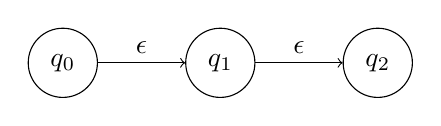
\begin{tikzpicture}[node distance=2cm,on grid,auto] 
	     \node[state] (q_0) {$q_0$}; 
	     \node[state] (q_1) [right=of q_0] {$q_1$}; 
	     \node[state] (q_2) [right=of q_1] {$q_2$}; 	      
	     \path[->] 
	      (q_0) edge  node {$\epsilon$} (q_1)
	      (q_1) edge  node {$\epsilon$} (q_2); 
	  \end{tikzpicture}
	 
\item Verbinde die Zustände in der Form mit einer einzigen Kante:

	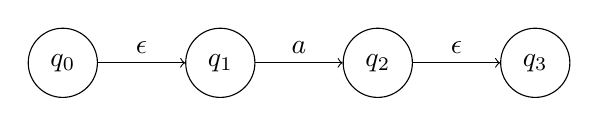
\begin{tikzpicture}[node distance=2cm,on grid,auto] 
	     \node[state] (q_0) {$q_0$}; 
	     \node[state] (q_1) [right=of q_0] {$q_1$};
	     \node[state] (q_2) [right=of q_1] {$q_2$};
	     \node[state] (q_3) [right=of q_2] {$q_3$};
	     \path[->] 
	      (q_0) edge  node {$\epsilon$} (q_1)
	      (q_1) edge  node {$a$} (q_2)
              (q_2) edge  node {$\epsilon$} (q_3);
	  \end{tikzpicture}
	  \\ wird zu

	  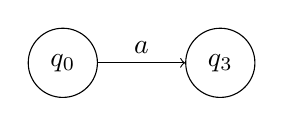
\begin{tikzpicture}[node distance=2cm,on grid,auto] 
	     \node[state] (q_0) {$q_0$}; 
	     \node[state] (q_3) [right=of q_0] {$q_3$}; 
	     \path[->] 
	      (q_0) edge  node {$a$} (q_3);
	  \end{tikzpicture}

\item Lösche nicht erreichbare Zustände
\item Falls $\epsilon$ in der Sprache ist, dann mache den Startzustand Endzustand
\end{enumerate}



\subsection{Reguläre Ausdrücke (REs)} % (fold)
\label{sub:reguläre_ausdrücke}

\begin{itemize}
  \item Reguläre Ausdrücke sind induktiv definiert:
\begin{itemize}
  \item $\emptyset$
\item $\epsilon$
\item Für jedes $a \in \Sigma$
\item Wenn $\alpha$, $\beta$ RE, auch:
	\begin{itemize}
		\item[-] $\alpha \beta$
		\item[-] $\alpha \ | \ \beta$ = $\alpha + \beta$
		\item[-] $\alpha^*$
	\end{itemize}


\end{itemize}

\item $*$, Kleene'sche Iteration

\item Für RE $\gamma$ ist die Sprache induktiv definiert:
	\begin{itemize}
	  \item $L(\emptyset) = \emptyset$
	  \item $L(\epsilon) = \{\epsilon\}$
	\item $L(a) = \{a\}$
\item $L(\alpha \beta) = L(\alpha)L(\beta)$
	\item $L(\alpha \ | \ \beta) = L(\alpha) \cup L(\beta)$
	\item $L(\alpha^*) = L(\alpha)^*$
	\end{itemize}
\item $\alpha \equiv \beta$ gdw.\ $L(\alpha) = L(\beta)$
\item \textbf{Rechenregeln über REs:}
	\begin{itemize}
	  \item \textbf{Null und Eins Lemma:}
		  \begin{itemize}
			  \item[-] $\emptyset \ | \ \alpha \equiv \alpha \ | \ \emptyset \equiv \alpha$
			  \item[-] $\emptyset \alpha \equiv \alpha \emptyset \equiv \emptyset$
			  \item[-] $\epsilon \alpha \equiv \alpha \epsilon \equiv \alpha$
			  \item[-] $\emptyset^* \equiv \epsilon$
			  \item[-] $\epsilon^* \equiv \epsilon$

		  \end{itemize}

\item \textbf{Assoziativität:}
	\begin{itemize}
		\item[-] $(\alpha \ | \ \beta) \ | \ \gamma \equiv \alpha \ | \ (\beta \ | \ \gamma)$
		\item[-] $\alpha (\beta \gamma) \equiv (\alpha \beta) \gamma$
	\end{itemize}

\item \textbf{Kommutativität:}
	\begin{itemize}
		\item[-] $\alpha \ | \ \beta \equiv \beta \ | \ \alpha$
	\end{itemize}

\item \textbf{Distributivität:}
	\begin{itemize}
		\item[-] $\alpha (\beta \ | \ \gamma) \equiv \alpha \beta \ | \ \alpha \gamma$
		\item[-] $(\beta \ | \ \gamma) \alpha \equiv \beta \alpha \ | \ \gamma \alpha$
	\end{itemize}

\item \textbf{Idempotenz:}
	\begin{itemize}
		\item[-] $\alpha \ | \ \alpha \equiv \alpha$
	\end{itemize}
	\end{itemize}


\item \textbf{Stern Lemma:}
	\begin{itemize}
		\item[-] $\epsilon \ | \ \alpha \alpha^* \equiv \alpha^*$
		\item[-] $\alpha^* \alpha \equiv \alpha \alpha^*$
		\item[-] $(\alpha^*)^* \equiv \alpha^*$
	\end{itemize}
\end{itemize}

\pagebreak

\subsection{RE $\rightarrow$ $\epsilon$-NFA} % (fold)
\label{sub:rE_rightarrow_epsilon_nFA}
\begin{enumerate}
	\item Wende folgende Ersetzungsregeln an
		\begin{figure}[h!]
		  \centering
		  \includegraphics[width=0.8\linewidth]{ersetzungretonfa.png}
		  \label{fig:ersetzungretonfa_png}
		\end{figure}

\item Wende folgende Transformationsregeln an
	\begin{figure}[h!]
	  \centering
	  \includegraphics[width=0.8\linewidth]{transformationsregel.png}
	  \label{fig:transformationsregel_png}
	\end{figure}
\end{enumerate}

\textit{\underline{Beispiel:}}
\begin{figure}[h!]
  \centering
  \includegraphics[width=0.5\linewidth]{retonfabeispiel.png}
  \label{fig:retonfabeispiel_png}
\end{figure}
\pagebreak
\subsection{$\epsilon$-NFA $\rightarrow$ RE} % (fold)
\label{sub:_epsilon_nFA_rightarrow_rE}

\begin{enumerate}
	\item Hat Startzustand $q_1$ eingehende Übergänge, füge einen neuen Startzustand $q_0$ mit einem $\epsilon$-Übergang nach $q_1$
	\item Füge einen neuen Endzustand $q_3$ und $\epsilon$-Übergänge nach $q_3$ von allen Endzuständen ($q_2$ in diesem Beispiel)

		\begin{figure}[h!]
		  \centering
		  \includegraphics[width=0.8\linewidth]{nfatoreschritt1.png}
		  \label{fig:nfatoreschritt1_png}
		\end{figure}

\item Wähle ein Zustand $q$, der weder Start- noch Endzustand ist
\item Eliminiere $q$, wende dabei folgende Regeln:
\begin{figure}[h!]
  \centering
  \includegraphics[width=0.7\linewidth]{nfatoreschritt2.png}
  \label{fig:nfatoreschritt2_png}
\end{figure}
\end{enumerate}

\textit{\underline{Beispiel:}}

\begin{figure}[h!]
  \centering
  \includegraphics[width=0.56\linewidth]{nfatorebeispiel1.png}
  \includegraphics[width=0.4\linewidth]{nfatorebeispiel2.png}
  \label{fig:nfatorebeispiel_png}
\end{figure}

\subsection{Ardens Lemma} % (fold)
\label{sub:fA_}
\begin{itemize}
\item Sind $A, B, X$ Sprachen mit $\epsilon \not\in A$, so gilt:
	\large
	\begin{equation*}
	\boxed{
	\begin{aligned}
X = AX \cup B \Longrightarrow X = A^* B	
	\end{aligned}
	}
	\end{equation*}
	\normalsize
	
	\item Sind $\alpha, \beta, X$ REs mit $\epsilon \not\in L(\alpha)$, so gilt:
\large
\begin{equation*}
\boxed{
\begin{aligned}
	X \equiv \alpha X \ | \ \beta \Longrightarrow X \equiv \alpha^* \beta 
\end{aligned}
}
\end{equation*}
\normalsize

\item \textbf{Bemerkungen:}
	\begin{itemize}
		\item $X \equiv X\alpha \ | \ \beta \Longrightarrow X \equiv \beta \alpha^*$
		\item $X \equiv \alpha X \ | \ \beta$ für $\epsilon \in L(\alpha)$
		\begin{itemize}
		\item hat \textbf{keine eindeutige Lösung}: jede Sprache $B \subseteq X$ ist Lösung
		  \item \textit{\underline{Beispiel:}} für $\alpha = \epsilon$ und $\beta = b$ kann $X = b$ oder $X = a \ | \ b$ oder $X = aba \ | \ b$
		\end{itemize}
	
	\item $X \equiv X \ | \ aX$
		\begin{itemize}
		  \item hat \textbf{keine eindeutige Lösung:} $X = \emptyset$ oder $X = \Sigma^*$ oder $X = a^*$
		\end{itemize}
	
		\item $X \equiv \alpha X$ für $\epsilon \not\in L(\alpha)$
			\begin{itemize}
			  \item hat \textbf{eine eindeutige Lösung:} $X = \emptyset$
			\end{itemize}
		\item $X \equiv \alpha X$ für $\epsilon \in L(\alpha)$
			\begin{itemize}
				\item hat \textbf{keine eindeutige Lösung:} $X = \Sigma^*$ oder $X = ab^*a$
			\end{itemize}

		\item $X \equiv aXb \ | \ \epsilon$
			\begin{itemize}
				\item hat \textbf{keine reguläre Lösung:} $X = L$ für $L = \{a^nb^n, n \ge 0\}$

			\end{itemize}
			\item $X \equiv abX \ | \ \epsilon$
			\begin{itemize}
			  \item hat \textbf{eine eindeutige Lösung:} $X = (ab)^*\epsilon = (ab)^*$
			\end{itemize}
	\end{itemize}

\end{itemize}

\subsection{FA $\rightarrow$ RE mittels Ardens Lemma} % (fold)
\label{sub:fA_rightarrow_rE}
\begin{enumerate}
  \item FA als Gleichungssystem schreiben 
\begin{itemize}
  \item für jeden Endzustand $X_f$ füge $X_f \equiv \epsilon$ ein
\item für jeden Zustand $X$ mit 
	
	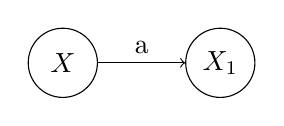
\begin{tikzpicture}[node distance=2cm,on grid,auto] 
	   \node[state] (X) {$X$}; 
	   \node[state] (X_1) [right=of X] {$X_1$}; 
	    \path[->] 
	    (X) edge  node {a} (X_1);
	\end{tikzpicture}

mache $X \equiv aX_1$
	
\end{itemize}

\item Gleichungen einsetzen und damit eliminieren
\item Rechenregeln über REs und Ardens Lemma verwenden
\end{enumerate}

\pagebreak

\subsection{Konversionen bezüglich regulärer Sprachen} % (fold)
\label{sub:konversionen_bezüglich_regulärer_sprachen}
\begin{figure}[h!]
  \centering
  \includegraphics[width=0.65\linewidth]{konversionregular}
  \label{fig:konversionregular}
\end{figure}



\subsection{Abschlusseigenschaften regulärer Sprachen} % (fold)
\label{sub:abschlusseigenschaften_regulärer_sprachen}
Seien $R, R_1, R_2 \subseteq \Sigma^*$ reguläre Sprachen, dann sind auch
\begin{itemize}
  \item $R_1 R_2$
\item $R_1 \cup R_2$, $R_1 \cap R_2$, $R_1 \setminus R_2$
\item $\overline{R}$ bzw. $\Sigma^* \setminus R$

\item $R^*$
\item $R^R$ (Spiegelung von $R$)
\end{itemize}

\subsection{Komplementierung $\overline{R}$ bezüglich FAs} % (fold)
\label{sub:komplementierung_bezüglich_fAs}
\begin{itemize}
  \item \textbf{Für DFAs:} Vertauschen von Endzuständen und Nicht-Endzuständen
\item \textbf{Für NFAs:} funktioniert das Vertauschen \textbf{nicht} 
\end{itemize}

\subsection{Schnitt zweier DFAs, Produktkonstruktion} % (fold)
\label{sub:produktkonstruktion}
\begin{itemize}
	\item Sind $M_1$ und $M_2$ DFAs. Dann ist der \textbf{Produkt-Automat} $\mathbf{M}$ mit $L(M) = L(M_1) \cap L(M_2)$.

	\item \textbf{Produktkonstruktion für $M_1$ und $M_2$:}
		\begin{enumerate}
			\item Erzeuge einen neuen Startzustand aus den Startzuständen der $M_1$ und $M_2$
			\item Bestimme wohin man mit welcher Kante geht
			\item Erzeuge neue Zustände durch Vereinigung der auf der rechten Seite stehenden Zuständen mit der selben Kanten, verbinde diese
			\item \textbf{Alle Zustände}, die in dem neuen Zustand sind, sind \textbf{Endzustände} $\rightarrow$ der neue Zustand wird ein Endzustand
		\end{enumerate}
\end{itemize}

\subsection{Vereinigung zweier DFAs} % (fold)
\label{sub:vereinigung_zweier_dFAs}
\begin{itemize}
\item Sind $M_1$ und $M_2$ DFAs. Dann ist $M$ mit $L(M) = L(M_1) \cup L(M_2)$.
\item \textbf{Konstruktion für $M_1$ und $M_2$:}
Gleich wie die Produktkonstruktion bis auf 4.
\begin{enumerate}
	\item[4.] \textbf{Mindestens einer von den Zuständen}, die in dem neuen Zustand sind, ist ein \textbf{Endzustand} $\rightarrow$ der neue Zustand wird ein Endzustand
\end{enumerate}
\end{itemize}

\subsection{Pumping Lemma für reguläre Sprachen} % (fold)
\label{sub:pumping_lemma}
\begin{itemize}
	\item Sei $L \subseteq \Sigma^*$ regulär. Dann gibt es ein $n > 0$, so dass sich jedes $z \in L$ mit $|z| \ge n$ so in $z = uvw$ zerlegen lässt, dass
\begin{enumerate}
  \item $v \neq \epsilon$
\item $|uv| \le n$
\item $\forall i \ge 0.$ $uv^iw \in L$
\end{enumerate}
  \item Um zu zeigen, dass eine Sprache \textbf{nicht regulär} ist $\rightarrow$ \textbf{Regulärität} mit Pumping Lemma zu zeigen \textbf{nicht möglich}
  \item Es gibt nicht-reguläre Sprachen, für die das Pumping-Lemma gilt \\$\rightarrow$ regulär $\subset$ Pumping Lemma gilt $\subset$ alle Sprachen

  \item \textit{\underline{Beispiel:}} $L = \{0^{m^{2}} \ | \ m \ge 0\}$
\\ \\ Angenommen $L$ sei regulär.
\\Sei $n$ eine Pumping-Lemma-Zahl für $L$.
\\Wähle $z = 0^{n^{2}} \in L$. Sei $uvw$ ist eine Zerlegung von $z$ mit $1 \le |v| \le |uv| \le n$.
\\ Zeige, dass $uv^iw \not\in L$ für den Fall $i = 2$ gilt:
\\ $n^2 = |z| = |uvw| < |uv^2w| \le n^2 + n \le n^2 + 2n + 1 = (n + 1)^2$
\\ Da es keine Quadratzahl zwischen $n^2$ und $(n+1)^2$ geben kann, ist $uv^2w \not\in L$, damit ist $L$ nicht regulär.


\end{itemize}

\subsection{Entscheidungsprobleme für reguläre Sprachen} % (fold)
\label{sub:entscheidungsprobleme_für_reguläre_sprachen}
\begin{itemize}
  \item \textbf{Wortproblem:} Gegeben $w$ und $D$, gilt $w \in L(D)$?
\begin{itemize}
	\item für DFA $M$, in $O(|w| + |M|\footnote{Konstante für die Entscheidung, ob der Zustand den wir am Ende erreichen, ein Endzustand ist})$ entscheidbar
\item für NFA $N$, in $O(|Q|^2|w| + |N|)$ entscheidbar
\end{itemize}

\item \textbf{Leerheitsproblem:} Gegeben $D$, gilt $L(D) = \emptyset$?
\begin{itemize}
	\item für DFA $M$, in $O(|Q||\Sigma|)$ entscheidbar
\item für NFA $N$, in $O(|Q|^2|\Sigma|)$ entscheidbar
\end{itemize}

\pagebreak

\item \textbf{Endlichkeitsproblem:} Gegeben $D$, ist $L(D)$ endlich?
\begin{itemize}
	  \item für DFA und NFA entscheidbar
	\item $L(M) = \infty$ gdw.\ vom Startzustand aus eine nicht-leere Schleife erreichbar ist, von der aus $F$ erreichbar ist
	\begin{figure}[h!]
	  \centering
	  \includegraphics[width=0.5\linewidth]{endlichkeitsproblem}
	  \label{fig:endlichkeitsproblem}
	\end{figure}
\end{itemize}

\item \textbf{Äquivalenzproblem:} Gegeben $D_1$ und $D_2$, gilt $L(D_1) = L(D_2)$?
\begin{itemize}
\item schaue, ob $L(M_1) \cap \overline{L(M_2)} = \emptyset$ und $\overline{L(M_1)} \cap L(M_2) = \emptyset$ gelten
	\item für DFAs, in $O(|Q_1||Q_2||\Sigma|)$ entscheidbar
	\item für NFA $N$, in $O(2^{|Q_1| +|Q_2|})$ entscheidbar (bei fixem $\Sigma$)
\end{itemize}\end{itemize}

\subsection{Minimierung von FAs} % (fold)
\label{sub:minimierung_der_fAs}





\end{document}
